%%% The main file. It contains definitions of basic parameters and includes all other parts.

%% Settings for single-side (simplex) printing
% Margins: left 40mm, right 25mm, top and bottom 25mm
% (but beware, LaTeX adds 1in implicitly)
\documentclass[12pt,a4paper]{report}
\setlength\textwidth{145mm}
\setlength\textheight{247mm}
\setlength\oddsidemargin{15mm}
\setlength\evensidemargin{15mm}
\setlength\topmargin{0mm}
\setlength\headsep{0mm}
\setlength\headheight{0mm}
% \openright makes the following text appear on a right-hand page
\let\openright=\clearpage

%% Settings for two-sided (duplex) printing
% \documentclass[12pt,a4paper,twoside,openright]{report}
% \setlength\textwidth{145mm}
% \setlength\textheight{247mm}
% \setlength\oddsidemargin{14.2mm}
% \setlength\evensidemargin{0mm}
% \setlength\topmargin{0mm}
% \setlength\headsep{0mm}
% \setlength\headheight{0mm}
% \let\openright=\cleardoublepage

\usepackage{amsmath}

%% Generate PDF/A-2u
\usepackage[a-2u]{pdfx}

%% Character encoding: usually latin2, cp1250 or utf8:
\usepackage[utf8]{inputenc}

%% Prefer Latin Modern fonts
\usepackage{lmodern}

%% Further useful packages (included in most LaTeX distributions)
\usepackage{amsmath}        % extensions for typesetting of math
\usepackage{amsfonts}       % math fonts
\usepackage{amsthm}         % theorems, definitions, etc.
\usepackage{bbding}         % various symbols (squares, asterisks, scissors, ...)
\usepackage{bm}             % boldface symbols (\bm)
\usepackage{graphicx}       % embedding of pictures
\usepackage{fancyvrb}       % improved verbatim environment
\usepackage{natbib}         % citation style AUTHOR (YEAR), or AUTHOR [NUMBER]
\usepackage[nottoc]{tocbibind} % makes sure that bibliography and the lists
			    % of figures/tables are included in the table
			    % of contents
\usepackage{dcolumn}        % improved alignment of table columns
\usepackage{booktabs}       % improved horizontal lines in tables
\usepackage{paralist}       % improved enumerate and itemize
\usepackage[usenames]{xcolor}  % typesetting in color

%%% Basic information on the thesis

% Thesis title in English (exactly as in the formal assignment)
\def\ThesisTitle{Thesis title}

% Author of the thesis
\def\ThesisAuthor{Martin Dráb}

% Year when the thesis is submitted
\def\YearSubmitted{2017}

% Name of the department or institute, where the work was officially assigned
% (according to the Organizational Structure of MFF UK in English,
% or a full name of a department outside MFF)
\def\Department{Name of the department}

% Is it a department (katedra), or an institute (ústav)?
\def\DeptType{Department}

% Thesis supervisor: name, surname and titles
\def\Supervisor{Petr Daněček}

% Supervisor's department (again according to Organizational structure of MFF)
\def\SupervisorsDepartment{department}

% Study programme and specialization
\def\StudyProgramme{study programme}
\def\StudyBranch{Software Systems}

% An optional dedication: you can thank whomever you wish (your supervisor,
% consultant, a person who lent the software, etc.)
\def\Dedication{%
Dedication.
}

% Abstract (recommended length around 80-200 words; this is not a copy of your thesis assignment!)
\def\Abstract{%
Abstract.
}

% 3 to 5 keywords (recommended), each enclosed in curly braces
\def\Keywords{%
{key} {words}
}

%% The hyperref package for clickable links in PDF and also for storing
%% metadata to PDF (including the table of contents).
%% Most settings are pre-set by the pdfx package.
\hypersetup{unicode}
\hypersetup{breaklinks=true}

% Definitions of macros (see description inside)
%%% This file contains definitions of various useful macros and environments %%%
%%% Please add more macros here instead of cluttering other files with them. %%%

%%% Minor tweaks of style

% These macros employ a little dirty trick to convince LaTeX to typeset
% chapter headings sanely, without lots of empty space above them.
% Feel free to ignore.
\makeatletter
\def\@makechapterhead#1{
  {\parindent \z@ \raggedright \normalfont
   \Huge\bfseries \thechapter. #1
   \par\nobreak
   \vskip 20\p@
}}
\def\@makeschapterhead#1{
  {\parindent \z@ \raggedright \normalfont
   \Huge\bfseries #1
   \par\nobreak
   \vskip 20\p@
}}
\makeatother

% This macro defines a chapter, which is not numbered, but is included
% in the table of contents.
\def\chapwithtoc#1{
\chapter*{#1}
\addcontentsline{toc}{chapter}{#1}
}

% Draw black "slugs" whenever a line overflows, so that we can spot it easily.
\overfullrule=1mm

%%% Macros for definitions, theorems, claims, examples, ... (requires amsthm package)

\theoremstyle{plain}
\newtheorem{thm}{Theorem}
\newtheorem{lemma}[thm]{Lemma}
\newtheorem{claim}[thm]{Claim}

\theoremstyle{plain}
\newtheorem{defn}{Definition}

\theoremstyle{remark}
\newtheorem*{cor}{Corollary}
\newtheorem*{rem}{Remark}
\newtheorem*{example}{Example}

%%% An environment for proofs

%%% FIXME %%% \newenvironment{proof}{
%%% FIXME %%%   \par\medskip\noindent
%%% FIXME %%%   \textit{Proof}.
%%% FIXME %%% }{
%%% FIXME %%% \newline
%%% FIXME %%% \rightline{$\square$}  % or \SquareCastShadowBottomRight from bbding package
%%% FIXME %%% }

%%% An environment for typesetting of program code and input/output
%%% of programs. (Requires the fancyvrb package -- fancy verbatim.)

\DefineVerbatimEnvironment{code}{Verbatim}{fontsize=\small, frame=single}

%%% The field of all real and natural numbers
\newcommand{\R}{\mathbb{R}}
\newcommand{\N}{\mathbb{N}}

%%% Useful operators for statistics and probability
\DeclareMathOperator{\pr}{\textsf{P}}
\DeclareMathOperator{\E}{\textsf{E}\,}
\DeclareMathOperator{\var}{\textrm{var}}
\DeclareMathOperator{\sd}{\textrm{sd}}

%%% Transposition of a vector/matrix
\newcommand{\T}[1]{#1^\top}

%%% Various math goodies
\newcommand{\goto}{\rightarrow}
\newcommand{\gotop}{\stackrel{P}{\longrightarrow}}
\newcommand{\maon}[1]{o(n^{#1})}
\newcommand{\abs}[1]{\left|{#1}\right|}
\newcommand{\dint}{\int_0^\tau\!\!\int_0^\tau}
\newcommand{\isqr}[1]{\frac{1}{\sqrt{#1}}}

%%% Various table goodies
\newcommand{\pulrad}[1]{\raisebox{1.5ex}[0pt]{#1}}
\newcommand{\mc}[1]{\multicolumn{1}{c}{#1}}


% Title page and various mandatory informational pages
\begin{document}
%%% Title page of the thesis and other mandatory pages

%%% Title page of the thesis

\pagestyle{empty}
\hypersetup{pageanchor=false}
\begin{center}

\centerline{\mbox{
\includegraphics[width=166mm]{img/logo-en.pdf}}}

\vspace{-8mm}
\vfill

{\bf\Large MASTER THESIS}

\vfill

{\LARGE\ThesisAuthor}

\vspace{15mm}

{\LARGE\bfseries\ThesisTitle}

\vfill

\Department

\vfill

\begin{tabular}{rl}

Supervisor of the master thesis: & \Supervisor \\
\noalign{\vspace{2mm}}
Study programme: & \StudyProgramme \\
\noalign{\vspace{2mm}}
Study branch: & \StudyBranch \\
\end{tabular}

\vfill

% Zde doplňte rok
Prague \YearSubmitted

\end{center}

\newpage

%%% Here should be a bound sheet included -- a signed copy of the "master
%%% thesis assignment". This assignment is NOT a part of the electronic
%%% version of the thesis. DO NOT SCAN.

%%% A page with a solemn declaration to the master thesis

\openright
\hypersetup{pageanchor=true}
\pagestyle{plain}
\pagenumbering{roman}
\vglue 0pt plus 1fill

\noindent
I declare that I carried out this master thesis independently, and only with the cited
sources, literature and other professional sources.

\medskip\noindent
I understand that my work relates to the rights and obligations under the Act No.~121/2000 Sb.,
the Copyright Act, as amended, in particular the fact that the Charles
University has the right to conclude a license agreement on the use of this
work as a school work pursuant to Section 60 subsection 1 of the Copyright Act.

\vspace{10mm}

\hbox{\hbox to 0.5\hsize{%
In ........ date ............	% FIXME!
\hss}\hbox to 0.5\hsize{%
signature of the author
\hss}}

\vspace{20mm}
\newpage

%%% Mandatory information page of the thesis

\openright

\vbox to 0.5\vsize{
\setlength\parindent{0mm}
\setlength\parskip{5mm}

Title:
\ThesisTitle

Author:
\ThesisAuthor

\DeptType:
\Department

Supervisor:
\Supervisor, \SupervisorsDepartment

Abstract:
\Abstract

Keywords:
\Keywords

\vss}

\newpage

%%% Dedication

\openright

\noindent
\Dedication

\newpage

\openright
\pagestyle{plain}
\pagenumbering{arabic}
\setcounter{page}{1}


%%% A page with automatically generated table of contents of the master thesis

\tableofcontents

%%% Each chapter is kept in a separate file
\chapter{The Algorithm}
\label{chap:the-algorithm}

Our algorithm takes a reference sequence and a set of reads as inputs, and outputs a VCF file containing all detected variants. Both inputs are read into memory during the initialization phase, there are no memory-saving optimizations employed. In other words, no index files are used for the input data.

The variant calling is done on region basis. The reference sequence is divided into regions of constant length (2000 bases by default), sometimes also referred as \textit{active regions} and with 25 \% overlap. Reads are assigned to individual regions according to their mapping position. All regions are called independently and in parallel. To detect the variants, the following steps are performed:
\begin{itemize}
\item the reference sequence covering the active region is transformed into a De Bruijn-like graph,
\item reads assigned to the active region are integrated into the graph,
\item the graph structure is pruned and optimized,
\item variants are extracted,
\item genotypes and phasing are determined,
\end{itemize}

\section{Input, Output and Preprocessing}
\label{sec:input-output-and-preprocessing}

The reference sequence is expected to be in the FASTA format and starting at position 1. In a typical scenario, the whole chromosome is provided as an input. The FASTA file may contain multiple distinct reference sequences (covering mutliple chromosomes). Reference sequences are processed one at a time which means that at most one sequence is present in memory at any moment. Only characters \texttt{A}, \texttt{C}, \texttt{G} and \texttt{T} are considered valid nucleotides. Other characters, such as \texttt{N} used to mask low-complexity regions, are treated as invalid and reference regions filled with them are not subject to variant calling.

The read set needs to be stored in a text file reflecting the SAM format. Presence of header lines is not required, all information is deduced from the reads. Since the algorithm does not perform any error correction on its own, the input reads must be corrected beforehand. The error correction is supported as a separate command of the tool implementing our algorithm. The correction method was adopted from the \texttt{fermi-lite}\cite{fermi-lite} project and Chapter \ref{chap:read-error-correction} describes it in detail.

After the whole SAM file is read into memory and parsed, reads considered useless for the purpose of variant calling are removed from the set. Contents of the \texttt{FLAGS} column of the SAM file serves as a main filter, since it is used to detect the following types of undesirable reads:
\begin{itemize}
\item \textbf{unmapped}, recognized by the bit 2 set to 1,
\item \textbf{secondary alignments}, detected by the bit 8 set to 1,
\item \textbf{duplicates}, bit 10 is set to 1,
\item \textbf{supplementary}, bit 11 is 1.
\end{itemize}

Also, reads with the mapping position (\texttt{POS}) set to zero and with mapping quality (\texttt{MAPQ}) lower then certain threshold, defined to $10$ by default, are removed from the set. Read's mapping quality is also used to update individual base qualities. Each base quality $q$ is updated according to the formula
$$
q = min(q, MAPQ)
$$
Several other SAM fields play a role in read preprocessing. The \texttt{CIGAR} string is used to detect and remove soft-clipped bases. The \texttt{QNAME} values are used to detect paired end reads, \texttt{RNAME} gives the name of the input reference sequence (chromosome).

The SAM file format is described in great detail in \cite{sambam}.

When all the reads are preprocessed this way, they are assigned to that respective active regions based on the mapping position. Then, the main algorithm comes into play.

\section{K-mer Representation}
\label{sec:kmer-representation}

Our algorithm works with k-mers only through an interface consisting from several functions and macros. The k-mer implementation is used as a blackbox which allows us to make several implementations and then choose the best fitting one without any consequences on the rest of the algorithm, exceptthose implied by the interface.

We currently use two implementations representing k-mers in different ways, shown on Figure \ref{fig:kmer-representations}. For performance reasons, the implementations may be switched only in compile time. 

The upper part of the figure shows the representation of the \textit{debuging} k-mer. The main idea behind this type of k-mer is to make the content easily human-readable, which is excellent for debugging purposes. The k-mer sequence is stored in a character array, each element represents one base. Except its context number, the purpose of which is explained in the next section, each debug k-mer also remembers its size. That value is used for debugging purposes only, mainly to recognize attempts to pass wrong k-mer size arguemnt to one of the k-mer interface routines. Debug k-mers also have an advantage of potentialy unlimited maximum size. It is clear that debug k-mers are not a good option in terms of performance, especially for bigger $k$.

\textit{Compact}, k-mers in contrast,  are more optimized for performance and quick append and prepend operations (moving the k-mer sequence forward or backward). Their design is greatly inspired by the k-mer implementation of the \texttt{fermi-lite} project. The k-mer sequence is stored in three 64-bit integers. Each base is represented by three bits, each stored separately in  the three integer fields. To read a $i^{th}$ base (starting from zero), one needs to combine $(k-i-1)^{th}$ bits of the integers and then translate the result by rules described in Table \ref{tab:base-translation}. The table also describes the meaning of the eight possible values.

Structure of a compact k-mer is displayed in lower part of Figure \ref{fig:kmer-representations}. Its advantages are a fixed size of 28 bytes for all k-mer sizes and performance. However, limiting the maximum k-mer size to 63 bases this way may impose a problem in case of assembling repetitive regions.

\begin{table}[h]
\begin{center}
\caption{Base representations in debugging and compact k-mers}
\label{tab:base-translation}
\begin{tabular}{| c | c | p{5cm} |}
\hline
Compact value & Debugging value & Meaning \\
\hline
0 & \texttt{A} & The base \texttt{A} \\
\hline
1 & \texttt{C} & The base \texttt{C} \\
\hline
2 & \texttt{G} & The base \texttt{G} \\
\hline
3 & \texttt{T} & The base \texttt{T} \\
\hline
4 & \texttt{B} & Denotes beginning and and of the active region. \\
\hline
5 & \texttt{H} & Used to represent k-mers of helper vertices. \\
\hline
6 & \texttt{D} & Used to represent k-mers of helper vertices. \\
\hline
7 & \texttt{N} & - \\
\hline
\end{tabular}
\end{center}
\end{table}

\begin{figure}[h]
	\centering
	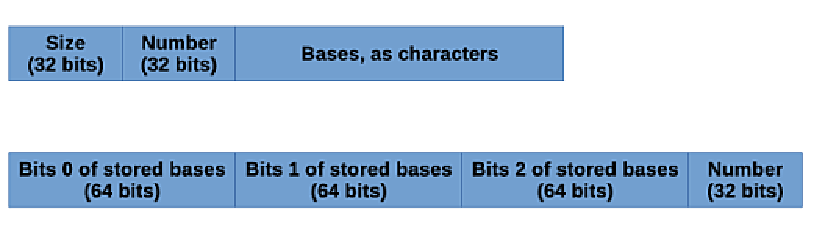
\includegraphics{img/kmer-representations}
	\caption{Two possible k-mer representations used by our algorithm; debugging (the upper part) and compact (the lower part).}
	\label{fig:kmer-representations}
\end{figure}

All k-mer implementations usable by our algorithm must reserve some space for storing a \textit{k-mer context number}. The number is used to differentiate even between k-mers that contain the same substring of length $k$. That implies that a k-mer, according to this new definition, is unique only if it differs in both the substring and the context number from all other k-mers. K-mers that differ only in the context number are sometimes referred as \textit{equal by (sub)string} or \textit{equal by sequence}. The context number proves to be useful when fighting repeats within the reference sequence (described in Section \ref{sec:reference-transformation}).

\textbf{The whole chapter uses the term k-mer in this sense described above, unless explicity specified otherwise}.

The \texttt{fermi-lite} project uses two bits to represent each base in the k-mer. Our algorithm can be modified to do the same, since the helper vertices actually do not need k-mers and exist mostly for the sake of code simplicity (no special handling regarding helper vertices is required). Similarly, there is no real reason for marking beginning and end of the active region by a special character, this was only useful for debugging.

\section{Reference transformation}
\label{sec:reference-transformation}

The first step of the algorithm lies in transforming a reference sequence covering the selected active region into a de Bruijn-like graph. The idea behind this step is very similar to other assembly algorithms based on these graph types. 

The reference is decomposed into k-mers, each overlaps with the adjacent ones by $k-1$ bases. K-mers representing the same sequence are differentiated by their context number, so each k-mer derived from the reference is unique. Two extra k-mers, denoting the beginning and the end of the active region are added to the set. Then, each k-mer is represented by a single vertex in the graph, and edges are defined by the order of the k-mers within the reference.

Formaly speaking, with the active region of length $l$ represented as a string $b_1 \ldots b_{l}$, k-mers $k_0, ..., k_{l-k+2}$ are derived from the region as follows:
\begin{itemize}
\item $k_0 = (Bb_1 \ldots b_{k-1}, 0)$
\item $k_1 = (b_1 \ldots b_k, 0)$
\item . . .
\item $k_i = (b_i b_{i+k-1}, c_i), 2 \leq i \leq  l-k+1$
\item . . .
\item $k_{l-k+2} = (b_{l-k+2} \ldots b_lB) 0)$
\end{itemize}
$c_i$ represents the context number of the k-mer $k_i$. The number is set to zero for k-mers unique within the active region. On the other hand, let's assume that k-mers $k_{i_1}, ..., k_{i_n}, i_0 < ... < i_n$, contain the same string. Their context numbers are defined as
$$
c_{i_j} = j, 
$$
$k_0$ and $k_{l-k+2}$ are special k-mers added to the set in order to show the start and end of the active region within the graph. \texttt{B} is a virtual base that ensures these k-mers are unique. The bases must not appear anywhere else within the active region. All k-mers created in this step and all vertices created from them are also called as \textit{reference k-mers} and \textit{reference vertices}. Similarly, k-mers and vertices created during the read integration phase, are sometimes referred as \textit{read k-mers} and \textit{read vertices}.

Each k-mer $k_i$ is transformed into a single vertex $v_i$. Edges follow the order of the k-mers in the active region. In other words, the edge set of the graph is
$$
E = \{(v_i, v_{i+1})\}\quad 0 \leq i \leq l-k+1
$$
Figure \ref{fig:ref-my} displays a graph created by transforming the active region \texttt{ATCTGTATATATG} with k-mer size of 5. The algorithm creates the following k-mers:
\begin{align}
k_0 = (BATCT, 0) \\
k_1 = (ATCTG, 0) \\
k_2 = (TCTGT, 0) \\
k_3 = (CTGTA, 0) \\
k_4 = (TGTAT, 0) \\
k_5 = (GTATA, 0) \\
k_6 = (TATAT, 0) \\
k_7 = (ATATA, 0) \\
k_8 = (TATAT, 1) \\
k_9 = (ATATG, 0) \\
k_{10} = (TATGB, 0)
\end{align}
As can bee seen, there are two k-mers representing sequence \texttt{TATAT}, namely $k_6$ and $k_8$. Because of their distinct context numbers, they are represented as separate vertices. Introduction of the context numbers removed a loop from the graph. The loop can be observed on Figure \ref{fig:ref-db} that shows a standard de Bruijn graph constructed from the same active region. K-mers $k_6$ and $k_8$ are represented by the same vertex. In order to recover the sequence, it is required to know how many times the loop was actually used during the transformation step.

\begin{figure}[h]
	\centering
	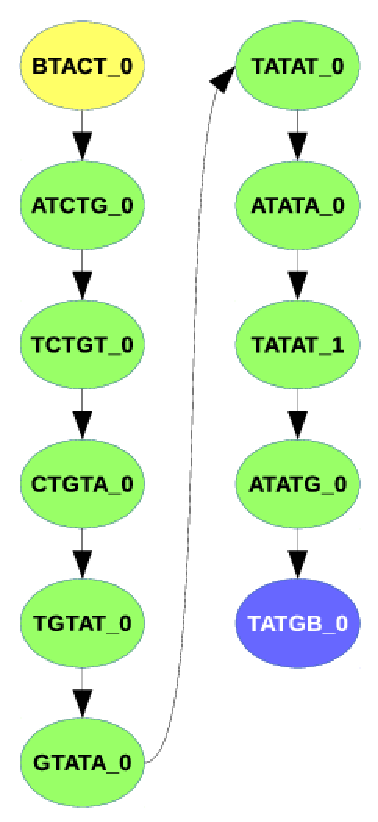
\includegraphics{img/ref-my.pdf}
	\caption{Graph resulting from the transformation of \texttt{ATCTGTATATATG} sequence}
	\label{fig:ref-my}
\end{figure}

\begin{figure}[h]
	\centering
	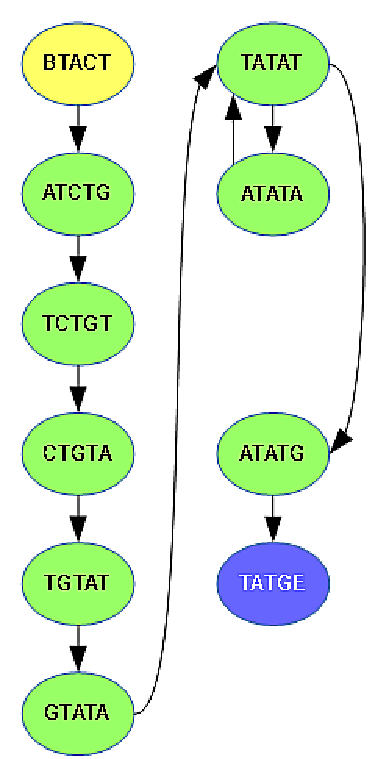
\includegraphics{img/ref-db.pdf}
	\caption{Transformation of the ATCTGTATATATG squence to a standard De Bruin graph (with no k-mer context numbers)}
	\label{fig:ref-db}
\end{figure}

Although this solves the problem of cycles for now, at least for now, things become more complicated in the next step of the algorithm which inserts individual reads into the graph

\section{Adding Reads}
\label{Adding Reads}

The basic idea behind this stage is farily simple and similar to the approach used in the previous one. The read being added is divided into a sequence of k-mers. If a k-mer is not represented by any existing graph vertex, a new vertex is created for it. In other cases, existing vertices are used. Again, vertices representing adjacent k-mers in the read are connected by edges. 

Figure \ref{fig:read-idea} shows a graph created by transforming a region of \texttt{ACCGTGGTAAT} and adding a read \texttt{ACCGTAGTAAT} to the resulting graph. K-mer size is set to 5. The read is divided into the following k-mers:
\begin{gather}
k_0 = ((A, C, C, G, T), 0) \\
k_1 = ((C, C, G, T, A), 0) \\
k_2 = ((C, G, T, A, G), 0) \\
k_3 = ((G, T, A, G, T), 0) \\
k_4 = (T, A, G, T, A), 0) \\
k_5 = ((A, G, T, A, A), 0) \\
k_6 = ((G, T, A, A, T), 0)
\end{gather}

In the graph, there already are vertices representing k-mers $k_0$ and $k_6$. For others, new vertices are created. Finally, edges are added (if necessary) to show the k-mer order within the read. The figure also suggests how to retrieve the sequence covered by the read --- just by following the edges and using the last base of all the k-mers except the first one that is used as a whole. 

\begin{figure}[h]
	\centering
	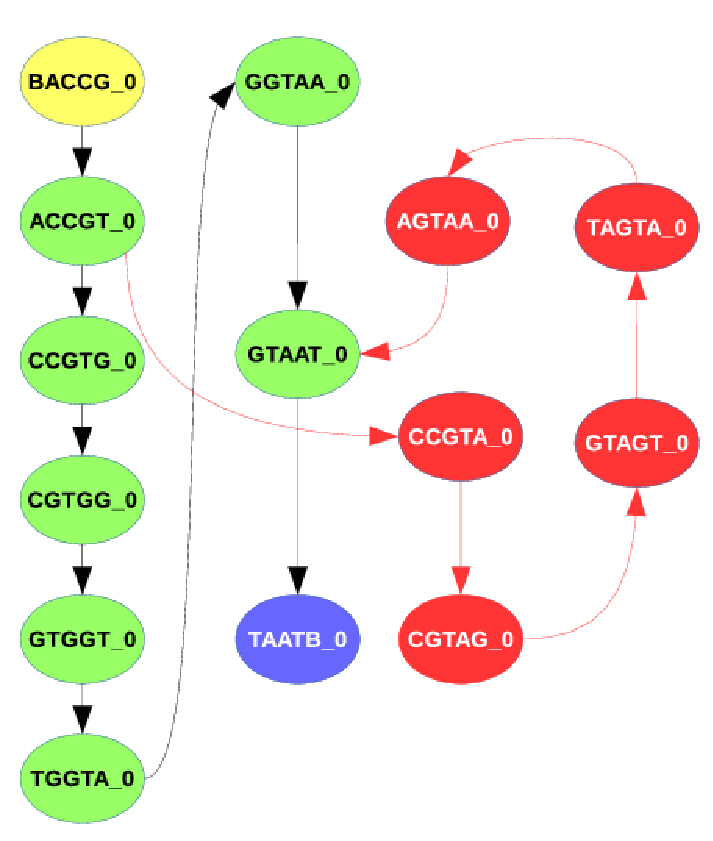
\includegraphics{img/read-idea.pdf}
	\caption{Basic idea behind adding a read into a De Bruin graph}
	\label{fig:read-idea}
\end{figure}

Figure \ref{fig:read-idea} reflects an ideal state, meaning that all places, where the read differs from the reference, are covered by distinct k-mers, and distance between each two of them is greater than $k$. If these conditions are met, each single $n$-base long difference (SNP, insertion or deletion) adds atmost $n+k-1$ new vertices to the graph. However, it may happen that some of the k-mers covering a difference colide by sequence with either k-mers of the reference, or k-mers of other reads covering a totally different place of the active region. To minimize such unfortunate cases, additional graph transformations need to be made after all the reads are added to the graph.

Unfortunately, the basic idea does not work in our case. Introduction of the k-mer context numbers prevented loops in the graph derived purely from the reference. But since multiple k-mers representing the same sequence may exist, it is not always possible to easily determine which of the vertices should be assigned to individual k-mers of the read. For example, if looking at the graph from Figure \ref{fig:ref-my}, it is not clear which vertex (or vertices) should be assigned to a k-mer with \texttt{TATAT} sequence. 

We decided to solve the issue by transforming the basic idea into the following steps:
\begin{itemize}
\item divide the read into sequence of k-mers (a so-called \textit{short variant optimization}, described later, may be applied),
\item assign a set of vertices to each k-mer, so that all vertices in the set represent k-mers euqal to the read k-mer by sequence,
\item from each set, select a vertex to represent the k-mer of the read,
\item connect the vertices representing the read to respect the order of the k-mers in the read.
\end{itemize}

\subsection{Transforming the Read into K-mers}
\label{subsec:transforming-the-read-info-k-mers}

Let's define a read of length $n$ as a sequence $(r_1, ..., r_n)$ of bases. If the short variant optimization is not applied, the sequence is divided into individual k-mers $k_1, ..., k_{n-k+1}$ in the same way as for the reference case, except that no extra k-mers to denote read start and end are created. The k-mers look as follows:
\begin{gather}
k_0 = ((r_1, ..., r_k), 0) \\
... \\
k_{n-k+1} = ((r_{n_k+1}, ...,r_n), 0)
\end{gather}

Then, the step described in Subsection \ref{subsec:assign-sets} is applied.

As described in \ref{subsec:idea}, in an ideal case, an $n$-base long difference from the reference produces $n + k - 1$ k-mers different from all reference k-mers. To reduce the probablity that some of the k-mers actually colide with either the reference, or another read, the \textit{short variant optimization} may be applied. The optimization reduces the number of k-mers representing a $n$-base long difference to:
\begin{itemize}
\item $n$ for an insertion,
\item zero for a deletion,
\item $1$ for a SNP.
\end{itemize}

The optimization assumes that when recovering a sequence from the graph, only the last base of each k-mer, wth an exception of the starting one, is used. So, only k-mers covering the difference by their last base need to be added; reference k-mers may be used for the rest in case the difference is followed by a reasonable number of bases equal to the reference. 

Figure \ref{fig:read-optimization} shows how the graph is optimized for a read containing SNP. The reference and read sequences are taken from Figure \ref{read-idea}. Since the difference has 1 base in length, only one k-mer (\texttt{CCTGA\_0}) is used to represent it. The k-mer is followed by reference k-mers. As can be seen, their last base are equal to one of k-mers from Figure \ref{read-idea}.

\begin{figure}
	\centering
	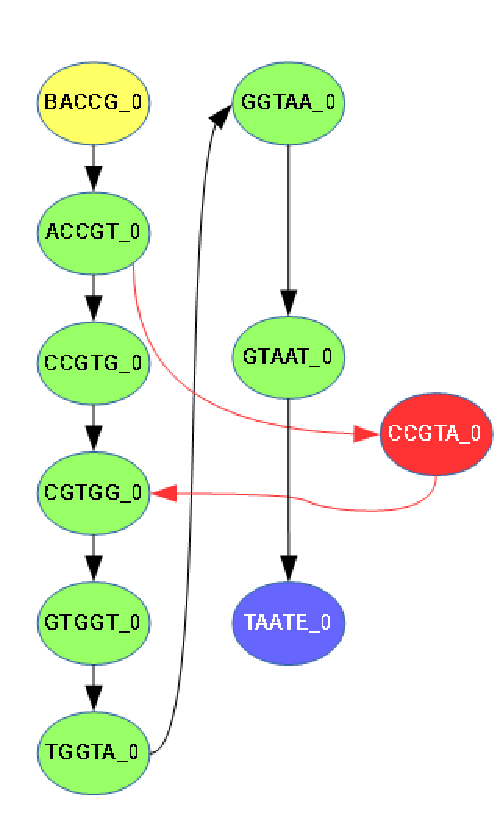
\includegraphics{img/read-optimization.pdf}
	\caption{Short Variant optimization}
	\label{fig:read-optimization}
\end{figure}

The short variant optimization is applied for k-mer $k_i$ if the following holds:
\begin{itemize}
\item There is only one reference vertex with a k-mer equal to $k_{i-1}$ by sequence. Let's assume this is vertex $v_{j-1}$
\item There is at most one vertex for $k_i$ that either is a result of a read addition, or is a reference one but do not immediately follows  the vertex $v_{j-1}$ in the reference.
\end{itemize}
Such conditions are met when the read differs from the reference at base $r_{i+k-1}$. To determine whether the difference is only a short one, the Smith-Waterman algorithm is applied. If this is the case, the action depends on the difference type:
\begin{itemize}
\item for $n$-base long deletion, $k_i$ is defined as $v_{j + n - 1}$,
\item for insertion of length $n$, $k_i$, ..., $k_{i + n - 1}$ are defined as with no short variant optimization and $k_{i + n}$ is set to $v_j$,
\item for SNP, $k_i$ is left as such and $k_{i+1}$ is defined as $v_{j+1}$
\end{itemize}

\subsection{Assigning Sets of Vertices to K-mers}
\label{subsec:assign-sets}

The process of assigning vertex sets to individual k-mers derived from the read in the previous step is quite straightforward --- a set assigned to certain k-mer $x$ contains exactly the vertices representing k-mers with sequence equal to $x$. The k-mer context number is not taken into account. If a k-mer is not represented by any vertex of the current graph (thus, the k-mer would receive an empty set), a new vertex is created to represent it. When using a standard De Bruin graph, size of all the sets would contain exactly one vertex and there would be merely anything to speak of. However, introduction of k-mer context numbers caused that also larger sets may appear. That decision, although removing loops from the reference vertices, complicates the task of integrating reads into the graph since the graph may contain multiple path representing a single read (by using differenct vertices with k-mers equal by sequence).

Previous steps of the algorithm, described above, impose the following conditions on the assigned vertex sets:
\begin{itemize}
\item each set contains either read, or reference vertices, not both,
\item if a set contains read vertices, its size is always one,
\item sets containing reference vertices do not have such restriction,
\item each two sets are either distinct (their intersection is an empty set) or equal.
\end{itemize}
The second and third condition holds because k-mer context numbers are used to differentiate reference k-mers but not the read ones. 

In formal terms, a set $M_i$ is assigned to a k-mer $k_i$ where
$$
M_i = {v_{i_j} | v_{i_j} \in V(G), kmer(v_{i_j}) equals to k_i by sequence}
$$ 
When a set is assigned to each k-mer, it is time to integrate the read into the graph in form of a path, starting on a vertex representing $k_1$ and ending in one covering $k_{n-k+1}$. SInce $M_i$ sets may contain more than one vertex, it is required to select vertices to form a path best fitting to the read. To derive a good path, we decided to honour the following observations about reads:
\begin{itemize}
\item they should follow the reference sequence in a forward direction,
\item probability of making big leaps in that direction is low,
\item multiple reads cover one place, sharing appropriate parts of their paths.
\end{itemize}

These observations cannot be enforced too strictly as De Bruin graphs are not very suitable for coping with repeats of length $k$ or more, and similar phenomenoms. The case of a read containing a copy of reference at leat $k$ baes in length might be enough to break the first observation. The second observation permits exceptions by definition. The third one forms a base for most of the genome assembly algorithms.

To solve the problem of selection of the right vertices from the $M_i$ sets, we decided to reduce it to a shortest-path problem on a helper graph the structure of which is defined by the sets and their contents.

\subsection{The Helper Graph}
\label{subsec:helper-graph}

The helper graph is an oriented layered one. Each layer consists of all vertices contained in one reference $M_i$ sets. The order of the layers respect the order of $M_i$ sets. Sets consisting of read vertices are not part of the helper graph. Only adjacent layers are connected by edges, their orientation reflects the order of the sets. Each subgraph consisting of two adjacent layers is a full bipartite graph. The structure of the helper graph does not take equality of $M_i$ into account. In other words, when $M_i = M_j$ for $i \ne j$, both sets are represented within the helper graph as individual layers, even if they refer to the same vertices of the (main, non-helper) graph.

Formaly speaking, let $M_i = \{v_{i}^{1}, ..., v_{i}^{n_i}\}$ and let $i$ serves as an index to reference sets only. Then the helper graph $G_h$ can be defined as follows:
\begin{gather}
G_h = (V_h, E_h) \\
V_h = \cup_i M_i \\
E_h = \{(u, v) | u \in M_i, v \in M_{i + 1}\}
\end{gather}

By finding the shortest path leading from a vertex in the first layer to one in the last layer, we perfrom the process of selection of vertices representing the read in the main graph. The shortest path depends on weights of edges connecting the adjacent layers. In general, the weighting function follows these rules:
\begin{itemize}
\item the weight is increased by a \textit{missing edge penalty} if there is a missing edge on the path from $u$ to $v$ in the main graph,
\item the weight is increased by a \textit{reference backward penalty} if reference position of $u$ is greater or equal to the reference position of $v$,
\item the weight is increased by a \textit{reference forward penalty} if reference psotiion of $u$ is far less than reference position of $v$.
\end{itemize}
The rules actually indicate why $M_i$ sets covering read vertices are not parts of the helper graph – since their vertices maintain no reference position, only the missing edge penalties would apply and that can be included within missing edge penalties of the reference vertices only.

For an example of a helper graph, let's have a reference sequence \texttt{ACTATACTA} and a read \texttt{ACTAGACTA}. The left part of Figure \ref{fig:heper-graph-short} shows the main graph just after adding vertices for the reference and the read k-mers with short variant optimization applied. The resulting helper graph is shown on the right part of the figure.

Six k-mers are derived from the read which means that vertex sets $M_0$, ..., $M_5$ are assigned to them. Since the second k-mer is represented by a read vertex, the $M_1$ set is not included as a layer of the helper graph. Other sets contains reference vertices, so they form individual layers. Adjacent layers are then connected. Edges with applied penalties (only the reference backward penalty in this case) are depicted red. The black edges show the shortest path.

\begin{figure}[h]
	\centering
	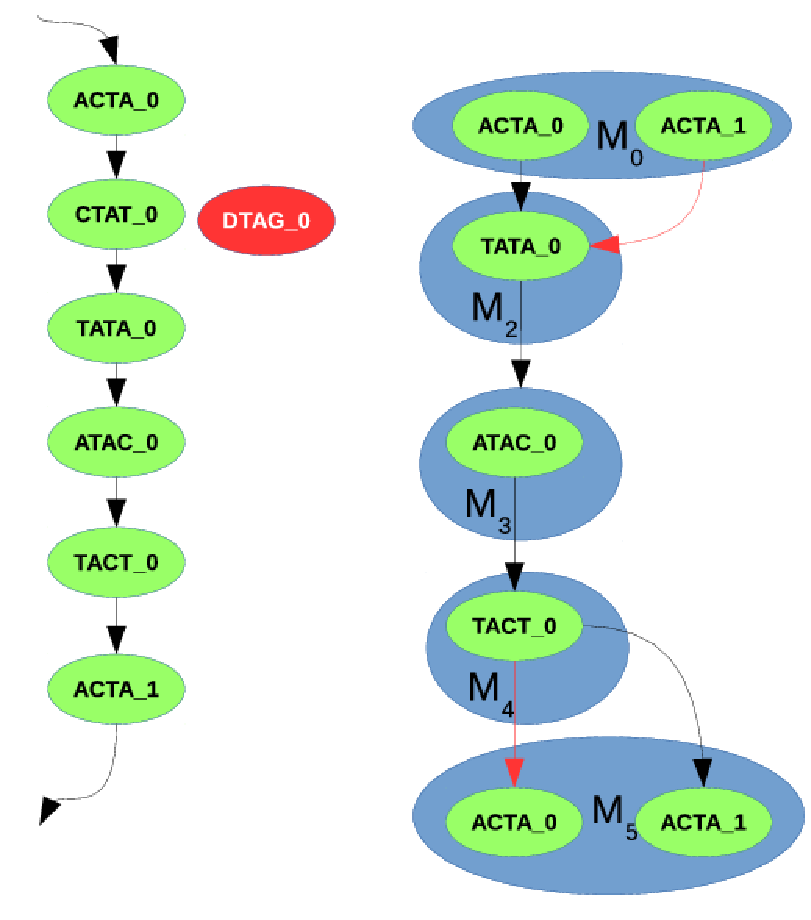
\includegraphics{img/helper-graph-short.pdf}
	\caption{Helper graph creation with short variant optimization}
	\label{fig:helper-graph-short}
\end{figure}

The shortest path select the first vertex from $M_0$ and the second one from $M_5$ to represent the read within the main graph (since other sets contain only one vertex, the selection process is trivial there). The resulting path in the graph can be used to correctly recover the sequence covered by the read.

As Figure \ref{fig:helper-graph} indicates, both graphs look a little bit differently when the short variant optimization is not applied. The main graph contains more read vertices which reduces the number of layers in the helper graph. Although the graphs are different, the sequence covered by the rad is the same and can be correctly recovered again.

\begin{figure}[h]
	\centering
	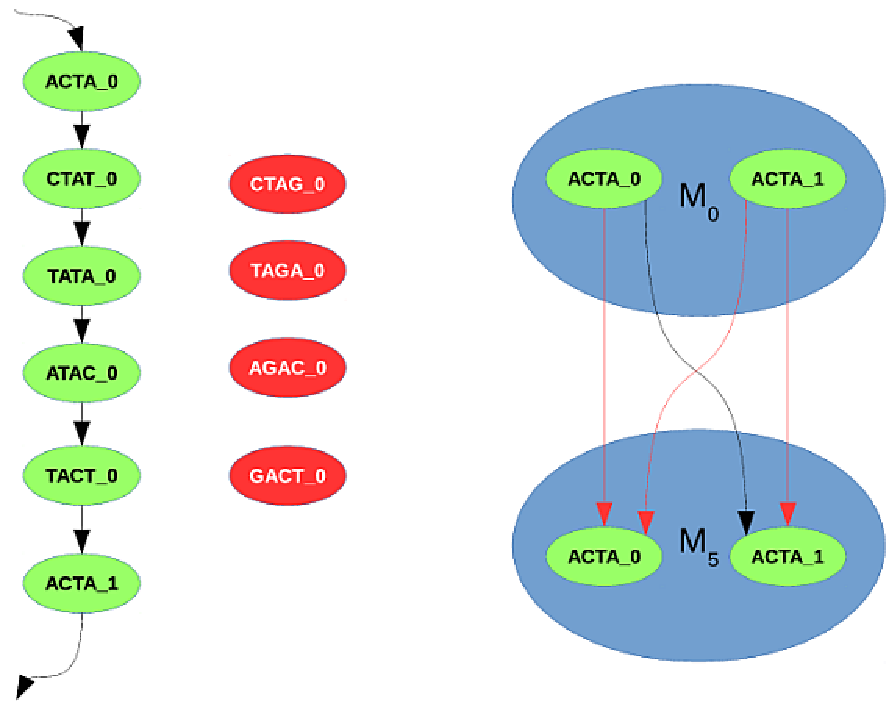
\includegraphics{img/helper-graph.pdf}
	\caption{Helper graph creation without short variant optimization}
	\label{fig:helper-graph}
\end{figure}

\section{Graph Structure Optimization}
\label{sec:graph-structure-optimization}

When all reads are integrated into the De Bruin-like graph, it is time to optimize its structure in order to get rid of unpopulated paths, usually created by read errors, and resolve some other issues caused mostly by repetitive regions inside either the reference or the reads.

\subsection{Connecting Bubbles}
\label{subsec:connecting-bubbles}

Figure \ref{fig:bubble-connection} demonstrates one class of the structural problems. A subset of reference sequence was transformed into vertices 1, 2, 3, 4, 5 and 6. A set of reads is represented by a "path" 2, 3, 4, 5, R1, R2, 1, 2, 3, R3, 6.  The left part of the figure shows how such a graph woud look like without any optimizations. It is clear that recovering the correct sequence would not be trivial. 

Howerver, since we know that the path leads from R2 to R3 (through 1, 2, 3), we can theoretically replace edges (R2, 1) and (3, R3) by a special edge (R2, R3), as the right part of the figure suggests. An information about the sequence covered by vertices 1 and 2 needs to be recorded within the new edge. Recovering the correct sequence from the right part of the figure does not impose a problem since it is just a simple bubble. 

\begin{figure}
	\centering
	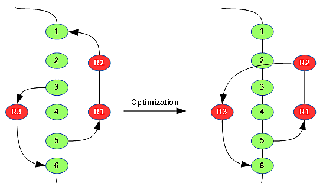
\includegraphics{img/bubble-connection.pdf}
	\caption{Benefits of connecting bubbles}
	\label{fig:bubble-connection}
\end{figure}

A more general, and a very typical, sutiation is shown on Figure \ref{fig:connection-general}. The subgraph contains a subset of the reference (vertices $1$, $...$, $n+1$) and two bubbles; one ending by $R1$ and connected to $2$, another starting at $R2$ and leading from $n$. If edges $I_1$ (the input edge) and $O_1$ (the output edge) share reasonable amount of reads ($|reads(I_1) \cap reads(O_1)| > thershold$), the subgraph may also be interpreted as that the reads contain a sequence of length $n-1$ that is also present in the reference. In that case, it is wise to connect the vertices $R1$ and $R2$ directly the same way as on Figure \ref{bubble-connection}, bypassing the reference part. The edge maintaining the direct link is marked as $C_1$ (the connecting edge). Reads shared by the input and the output edges are moved to the connecting one.

If $C_1$ is created, the read set intersection is also used to decide whether the edges $I_1$ and $O_1$ should be removed. The input edge is deleted if does not share enough reads with the next reference edge (meaning there are no valid sequences leading through both these edges). Similarly, the output edge is deleted in case it does not share enough reads with the last reference edge (no valid paths goes through the edges).

\begin{figure}[h]
	\centering
	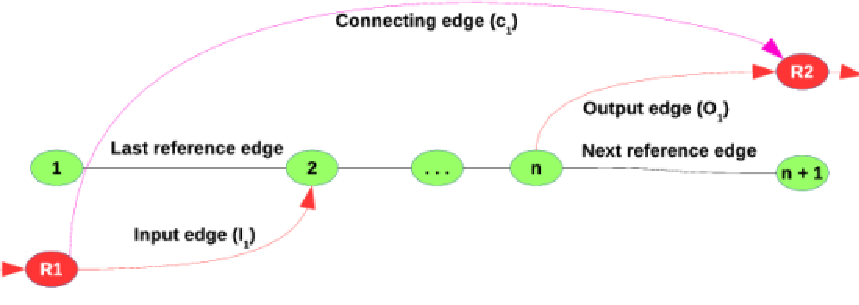
\includegraphics{img/connection-general.pdf}
	\caption{A subgraph required for connection}
	\label{fig:connection-general}
\end{figure}

Figure \ref{fig:connection-abstract} depicts probably the most general case; multiple reads covering different parts of the active region (including the differences from the reference) share the same sequence of $n$ bases. There is $k$ input and $l$ output edges. To determine the association between individual input and output edges, the intersection of covering reads is used again and connecting edges are created if necessary. More precisely, the following rules apply:
\begin{itemize}
\item If $i^{th}$ input and $j^{th}$ output edges share reasonable amount of reads ($|reads(I_i) \cap reads(O_j)| > threhsold$), a connecting edge $C_{i,j}$ is created and the shared reads are moved to it. The new edge starts in $source(I_i)$ and ends in $dest(O_j)$.
\item $I_i$ and $O_i$ are removed in case their read coverage drops below threshold as a result of moving it to the newly created $C_i$ edges. 
\end{itemize}

\begin{figure}[h]
	\centering
	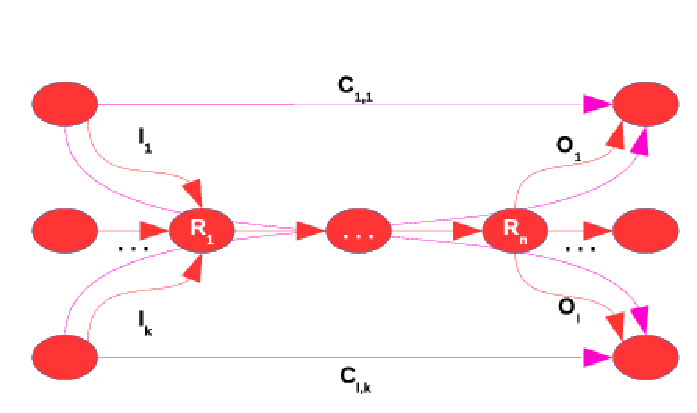
\includegraphics{img/connection-abstract.pdf}
	\caption{A general form of the subgraph}
	\label{fig:connection-abstract}
\end{figure}

\subsection{Helper Vertices}
\label{subsec:helper-vertices}

The bubble connection optimization works well when the bubbles being connected contain at least one read vertex. If this is not the case, howerver, the effect of replacing input and output edges with connection ones leads to a destruction of the sequences recorded within the graph.

As an example, consider a case ilustrated by the left part of Figure \ref{fig:helper-vertices}. The relevant part of the reference runs from vertex $1$ to $7$ and the read coverage supports a path of $3 \to 4 \to 5 \to 6 \to 1 \to 2 \to 4 \to 5 \to 7$. Applying steps described in this section leads into creating connection edges $6 \to 4$ and $2 \to 7$ and removing edges $6 \to 1$, $2 \to 4$ and $5 \to 7$. Such a graph cannot be used to recover the alternate sequence.

Since this problem appears only in case the bubbles are represented only by edges connecting reference vertices (the short variant optimization produces such cases for deletions), the countermeasure is quite straightforward; it lies in insertion of special vertices that presents themself as read ones but carry no information about the sequence on which path they exist. We use a conservative approach for their insertion which means they divide the following sorts of edges:
\begin{itemize}
\item output degree of their source vertex is greater than one,
\item input degree of their destination is greater than one.
\end{itemize}

The right part of Figure \ref{fig:helper-vertices} indicates where the helper vertices would be inserted. They divide edges $6 \to 1$, $2 \to 4$ and $5 \to 7$. If the bubble connection is applied now, it leads to creation of edges $H1 \to H2$ and $H2 \to H3$ and deletion of $H1 \to 2$, $3 \to H2$, $H2 \to 4$ and $5 \to H3$. The optimization caused the alternate sequence being recoverable ($3 \to 4 \to 5 \to 6 \to H1 \to H2 \to H3 \to 7$).

\begin{figure}[h]
	\centering
	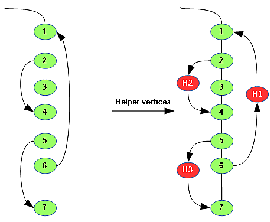
\includegraphics{img/helper-vertices.pdf}
	\caption{Use case for helper vertices}
	\label{fig:helper-vertices}
\end{figure}

\section{Variant Detection}
\label{sec:variant-detection}

The graph structure optimization phase ends by removing areas not covered enough by the input read set. Then, alternate sequences covered by the reads are recovered. Since the sequences share most of their parts with the reference, they are extracted in form of variants. Each variant describe one place of the reference where the alternate sequence differ which roughly corresponds to one line of a VCF file.

Variants are extracted by detecting certain subgraphs with preprogrammed interpretations. When such a subgraph is discovered, a variant is deduced from it and integrated back into the graph by replacing its reference edges by one \textit{variant edge}. Read edges unique to the variant are also removed from the subgraph which simplifies its structure. The process of variant detection stops when no suitable subgraphs are found.

Figure \ref{fig:variant-detection} shows four types of subgraphs used for variant extraction and how the extraction changes them. Requirements on the reference part are always the same; it must consist of a path starting in vertex \texttt{1}, ending in \texttt{n} and with all inner vertices having only one input and one output edge. Only edges of reference or variant type may be present in the reference part. In all cases, this path is replaced with a variant edge, shown as blue, connecting directly \texttt{1} and \texttt{n}. All edges that are removed as a result of the extraction are plotted as discontinuous lines.

\begin{figure}[h]
	\centering
	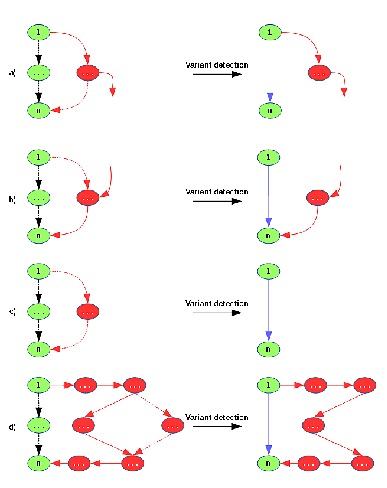
\includegraphics{img/variant-detection.pdf}
	\caption{Variant detection cases}
	\label{fig:variant-detection}
\end{figure}

\subsection{Simple Bubble}
\label{subsec:simple-bubble}

Read edges and vertices form a linear path leading from \texttt{1} to \texttt{n}. Since the edges are not part of any other variant, they all are removed and the whole subgraph degenerates only to two reference vertices connected by a variant edge. Figure \ref{variant-detection} shows this case under the \textbf{c)} sign.

\subsection{Bubble with Inputs}
\label{subsec:bubble-with-inputs}

Displayed under the \textbf{a)} sign, this sort of subgraphs differ from the simplest one only by allowing inut degree of the read vertices to reach above one. However, the restriction on the output degree remains in effect. Only the string of read edges leading from the \texttt{1} vertex to the first vertex with more inputs than one are removed. Other read edges may take part also in other variants.

\subsection{Bubble with Outputs}
\label{subsec:bubble-with-outputs}

This subgraph may be viewed as an opposite to the bubble with inputs. All read vertices in the subgraph are allowed to have more outputs than one, but only one input. Only the last string of edges, starting in the last read vertex with output greater than one and ending in the \texttt{n} vertex is removed, since it may participate only in one variant. The case is depicted under the \textbf{b)} sign of Figure \ref{fig:variant-detection}.

\subsection{Diamond}
\label{subsec:diamond}

The most complicated cae is shown under the \textbf{d)} letter and presents sort of a combination of a the \textbf{a)} and \textbf{b)} cases. The sequence of read vertices may contain one with output degree greater than one followed (not necessarily directly) by one with unresticted input degree. Only the edges covering one part of the supposed diamond are present in one variant only and hence are removed. 

\section{Varinat Graph and Variant Filtering}
\label{sec:variant-graph-and-variant-filtering}

When variants are extracted from the De Bruin-like graph, they need to be filtered and their genotype and phasing computed. The DB-like graph is not used to help with these tasks. The problem of genotype and phasing is transformed into a sort of graph colouring problem. A so-called \textit{variant graph} is built for this purpose.

The variant graph represent each variant by two vertices; one for its reference and one for its alternate sequence. The final task is to colour each vertex by one of these colors:
\begin{itemize}
\item \textbf{Blue}. The variant part is used by the first sequence.
\item \textbf{Red}. The variant part is used by the second sequence.
\item \textbf{Purple}. Both sequences go through the variant part.
\end{itemize}

If a vetex is coloured purple, the vertex representing the other part of the variant is not required (no sequence goes through it) and is removed from the graph. The deletion usually happen only to the vertices representing the reference pats, since removing a vertex of the alternate path means that the variant was filtered out.

Before colouring, graph vertices are connected by several types of bidirectional edges that place vairous conditions on the colour of their sources and destinations.
\begin{itemize}
\item \textbf{Variant edges} connect vertices representing parts of one variant. Their source and destination must be coloured differently.
\item \textbf{Read edges} connect variant parts covered by the same subset of reads, such vertices need to be coloured by the same colour, with exception of purpole. If one of the vertices is purple, the other may get arbitrary color.
\item \textbf{Pair edge} put together variant parts that are covered by paired reads. They place the same conditions as read edges.
\end{itemize}

When the graph is coloured, the genotype and phasing information are known. The variants are written to the resulting VCF file.

%%% Bibliography
%%% Bibliography (literature used as a source)
%%%
%%% We employ bibTeX to construct the bibliography. It processes
%%% citations in the text (e.g., the \cite{...} macro) and looks up
%%% relevant entries in the bibliography.bib file.
%%%
%%% The \bibliographystyle command selects, which style will be used
%%% for references from the text. The argument in curly brackets is
%%% the name of the corresponding style file (*.bst). Both styles
%%% mentioned in this template are included in LaTeX distributions.

% \bibliographystyle{plainnat}    %% Author (year)
% \bibliographystyle{unsrt}     %% [number]
\bibliographystyle{ieeetr}

\renewcommand{\bibname}{References}

%%% Generate the bibliography. Beware that if you cited no works,
%%% the empty list will be omitted completely.
% \bibliography{References}

%%% If case you prefer to write the bibliography manually (without bibTeX),
%%% you can use the following. Please follow the ISO 690 standard and
%%% citation conventions of your field of research.

\begin{thebibliography}{99}

\bibitem{testreads} ftp://ftp.1000genomes.ebi.ac.uk/vol1/ftp/technical/pilot2\_high\_cov\_GRCh37\_bams/data/NA12878/alignment/

\bibitem{testref}
$http://ftp.1000genomes.ebi.ac.uk/vol1/ftp/technical/reference/human\_g1k\_v37.fasta.gz$

\bibitem{testvcf}
ftp://ftp.1000genomes.ebi.ac.uk/vol1/ftp/release/20130502/

\bibitem{rtgeval}
https://github.com/lh3/rtgeval

\bibitem{samtools}
http://www.htslib.org/

\bibitem{haplocall}
https://gatkforums.broadinstitute.org/gatk/discussion/4146/hc-step-2-local-re-assembly-and-haplotype-determination

\bibitem{dbg-apply}
Compeau, Phillip C., Pevzner, Pavel A., Tesler, Glenn:
How to apply de Bruijn graphs to genome assembly
Nature Biotechnology, Volume 29, Number 11, November 2011

\bibitem{alg-compare}
Li, Zhenyu, Chen, Yanxiang, Mu, Desheng, Yuan, Jianying, Shi, Yujian, Zhang, Hao, Gan, Jun, Li, Nan, Hu, Xuesong, Binghang Liu, Yang, Bicheng, Fan Wu:
Comparison of two major classes of assembly algorithms: overlap-major-consensus and de-bruijn graph
Advance Access, 19 December 2011

\bibitem{fermikit}
Li, Heng: FermiKit: assembly-based variant calling for Illumina resequencing data
Cornell University Library, 24. 4. 2015
https://arxiv.org/abs/1504.06574

\end{thebibliography}


%%% Figures used in the thesis (consider if this is needed)
\listoffigures

%%% Tables used in the thesis (consider if this is needed)
%%% In mathematical theses, it could be better to move the list of tables to the beginning of the thesis.
\listoftables

%%% Abbreviations used in the thesis, if any, including their explanation
%%% In mathematical theses, it could be better to move the list of abbreviations to the beginning of the thesis.
\chapwithtoc{List of Abbreviations}

%%% Attachments to the master thesis, if any. Each attachment must be
%%% referred to at least once from the text of the thesis. Attachments
%%% are numbered.
%%%
%%% The printed version should preferably contain attachments, which can be
%%% read (additional tables and charts, supplementary text, examples of
%%% program output, etc.). The electronic version is more suited for attachments
%%% which will likely be used in an electronic form rather than read (program
%%% source code, data files, interactive charts, etc.). Electronic attachments
%%% should be uploaded to SIS and optionally also included in the thesis on a~CD/DVD.
%%% Allowed file formats are specified in provision of the rector no. 23/2016.
\chapwithtoc{Attachments}

\openright
\end{document}

